\documentclass[11pt,a4paper]{article}

% ---------- Encodage & langue ----------
\usepackage[utf8]{inputenc}
\usepackage[T1]{fontenc}
\usepackage{lmodern}
\usepackage{babel}
\babelprovide[import,main]{french}
\usepackage{amsmath}

% ---------- Mise en page ----------
\usepackage[a4paper,top=2.5cm,bottom=2.5cm,left=2.5cm,right=2.5cm,headheight=14pt]{geometry}
\usepackage{graphicx}
\usepackage{xcolor}
\usepackage{fancyhdr}
\usepackage{lastpage}
\usepackage{enumitem}
\usepackage{booktabs}
\usepackage{tabularx}
\usepackage{array}
\usepackage{caption}
\usepackage{float}
\usepackage{listings}
\usepackage{amssymb}
\usepackage{pifont}
\usepackage{twemojis}
\usepackage{tcolorbox}
\usepackage[nolinks]{qrcode}
\usepackage{xurl}
\usepackage[hidelinks]{hyperref}

\definecolor{bordeaux}{HTML}{6D1A2B}
\definecolor{grisclair}{HTML}{7A6D6F}
\definecolor{fondcode}{HTML}{FBF8F7}
\definecolor{bordurecode}{HTML}{E4DAD9}
\definecolor{vertok}{HTML}{3F7A55}

% ---------- En-têtes / pieds de page ----------
\pagestyle{fancy}
\fancyhf{}
\fancyhead[L]{\small\color{grisclair}ISSAT Sousse --- Département Informatique}
\fancyhead[R]{\small\color{grisclair}Rapport Mini Projet Web --- FIA3}
\renewcommand{\headrule}{\color{bordeaux}\hrule height 0.6pt}
\fancyfoot[C]{\small\color{grisclair}Page \thepage\ / \textcolor{bordeaux}{\pageref*{LastPage}}}
\renewcommand{\footrulewidth}{0pt}

% ---------- Légendes ----------
\captionsetup{labelfont={bf,sc},labelsep=endash,font=small}
\captionsetup[lstlisting]{labelfont={bf,sc},labelsep=endash}
\renewcommand{\lstlistingname}{Code}

% ---------- Listes « tiret » ----------
\setlist[itemize]{label=---,leftmargin=1.6em,itemsep=2pt}

% ---------- Code ----------
\lstdefinelanguage{JavaScript}{
  keywords={const,let,var,function,return,if,else,for,new,class,constructor,this,try,catch,typeof,true,false,null,void},
  sensitive=true, comment=[l]{//}, morecomment=[s]{/*}{*/},
  morestring=[b]', morestring=[b]", morestring=[b]`
}
\lstdefinelanguage{CSS}{
  keywords={@media,@keyframes,from,to,!important},
  sensitive=false, morecomment=[s]{/*}{*/}, morestring=[b]", morestring=[b]'
}
\lstset{
  basicstyle=\ttfamily\footnotesize,
  keywordstyle=\color{bordeaux}\bfseries,
  commentstyle=\color{grisclair}\itshape,
  stringstyle=\color{vertok},
  numbers=left, numberstyle=\tiny\color{grisclair}, numbersep=8pt,
  backgroundcolor=\color{fondcode},
  frame=single, rulecolor=\color{bordurecode},
  breaklines=true, breakatwhitespace=false,
  postbreak=\mbox{\textcolor{grisclair}{$\hookrightarrow$}\space},
  showstringspaces=false, columns=fullflexible, keepspaces=true,
  tabsize=4, captionpos=b, xleftmargin=1.5em, framexleftmargin=1.5em,
  escapeinside={^}{^},
  extendedchars=true,
  literate=
    {é}{{\'e}}1 {è}{{\`e}}1 {ê}{{\^e}}1 {à}{{\`a}}1 {â}{{\^a}}1
    {ç}{{\c c}}1 {î}{{\^i}}1 {ï}{{\"i}}1 {ô}{{\^o}}1 {ù}{{\`u}}1
    {û}{{\^u}}1 {É}{{\'E}}1 {À}{{\`A}}1 {œ}{{\oe}}1
    {«}{{\guillemotleft}}1 {»}{{\guillemotright}}1
}

\newcommand{\capture}[3]{%
  \begin{figure}[H]
    \centering
    \fcolorbox{bordurecode}{white}{\includegraphics[width=#2]{../images/#1}}
    \caption{#3}
  \end{figure}}

\newcommand{\aremplacer}[2]{%
  \begin{figure}[H]
  \centering
  \begin{tcolorbox}[colback=fondcode,colframe=bordeaux,boxrule=0.8pt,arc=2mm,
                    width=0.9\linewidth,height=4.2cm,valign=center,halign=center]
    \textbf{\textcolor{bordeaux}{Capture à insérer}}\\[4pt]
    \small #1
  \end{tcolorbox}
  \caption{#2}
  \end{figure}}

\emergencystretch=3em
\begin{document}

% =========================================================
% PAGE DE GARDE
% =========================================================
\begin{titlepage}
\thispagestyle{empty}
\centering
{\bfseries République Tunisienne}\\[6pt]
Ministère de l'Enseignement Supérieur\\
et de la Recherche Scientifique\\[1.2cm]

\begin{minipage}{0.45\textwidth}\centering
  
\includegraphics[height=2.1cm]{../images/logo_uvt.jpg}
\end{minipage}\hfill
\begin{minipage}{0.45\textwidth}\centering
  
\includegraphics[height=2.1cm]{../images/logo_issat.jpg}
\end{minipage}\\[1.2cm]

{\bfseries Université de Sousse}\\[6pt]
{\bfseries Institut Supérieur des Sciences Appliquées}\\
{\bfseries et de Technologie de Sousse}\\[0.8cm]
{\bfseries DÉPARTEMENT INFORMATIQUE}\\[1.8cm]

\rule{\linewidth}{0.8pt}\\[0.4cm]
{\LARGE \textcolor{bordeaux}{RAPPORT DE MINI PROJET WEB}}\\[0.35cm]
{\large\bfseries Sujet 7 --- Page de Quiz interactif}\\[0.1cm]
{\normalsize\color{grisclair} Version 2 : niveaux de difficulté, meilleurs scores et thème sombre}\\[0.3cm]
\rule{\linewidth}{0.8pt}\\[1.6cm]

\begin{tabular}{@{}l@{\hspace{0.6cm}}l@{}}
  \textbf{Classe :} & FIA3 \\[8pt]
  \textbf{Titre du mini-projet :} & Quiz interactif --- « Quiz Tunisie » \\[8pt]
  \textbf{Élaboré par :} & Tlili Faten \quad Limam Hiba \\[8pt]
  \textbf{Année universitaire :} & 2026 / 2027 \\
\end{tabular}

\vfill
{\small\color{grisclair} Version responsive testée --- Thème clair \& sombre --- HTML5 / CSS3 / JavaScript (ES6)}
\end{titlepage}

\pagenumbering{roman}
\tableofcontents
\listoffigures
\clearpage
\pagenumbering{arabic}

% =========================================================
\section{Introduction}
% =========================================================
Dans le cadre du module de développement web du département Informatique de l'ISSAT
Sousse, nous avons été amenés à réaliser un mini-projet front-end en \textbf{HTML5},
\textbf{CSS3} et \textbf{JavaScript pur} (sans framework). Le sujet retenu est le
\textbf{Sujet 7 : Page de Quiz interactif}, dont l'objectif est de concevoir une interface
web ludique permettant de répondre à un quiz, avec affichage du score en temps réel et
feedback visuel immédiat sur chaque réponse.

L'application, intitulée « \textbf{Quiz Tunisie} », propose cinq catégories thématiques
(Histoire, Géographie, Informatique, Comédie, Culture générale) ainsi qu'un mode
\textbf{« Toutes catégories »} qui mélange l'ensemble des questions. Le joueur choisit
un \textbf{niveau de difficulté} (Facile, Moyen, Difficile) qui fixe le temps accordé par
question et le nombre de points. Chaque partie enchaîne cinq questions --- à choix multiples
(QCM) ou de type \textbf{Vrai / Faux} --- avant d'afficher un écran de résultats détaillé
comprenant un récapitulatif des erreurs.

Cette deuxième version du projet ajoute de nombreuses fonctionnalités par rapport à la
première : système de points avec bonus de rapidité, sauvegarde des meilleurs scores
(\texttt{localStorage}), explication après chaque réponse, raccourcis clavier, thème
sombre automatique et réorganisation du code JavaScript en classes.

Ce rapport présente successivement le cahier des charges, la conception (architecture,
charte graphique, outils), l'implémentation commentée, les résultats obtenus sous forme de
captures d'écran et de validation W3C, les améliorations apportées par rapport à la
première version, les difficultés rencontrées et les solutions apportées, puis une
conclusion et les annexes.

% =========================================================
\clearpage
\section{Cahier des charges / Objectifs}
% =========================================================
L'application devait répondre aux exigences suivantes :
\begin{itemize}
  \item proposer un écran d'accueil présentant les règles du jeu et les meilleurs scores ;
  \item permettre le choix parmi plusieurs catégories de questions, ou toutes à la fois ;
  \item permettre le choix d'un \textbf{niveau de difficulté} (Facile / Moyen / Difficile) ;
  \item générer aléatoirement cinq questions par partie, adaptées au niveau choisi, avec
        des réponses mélangées pour les QCM ;
  \item gérer deux types de questions : \textbf{QCM} (4 réponses) et \textbf{Vrai / Faux} ;
  \item lancer un chronomètre par question (20 s, 15 s ou 10 s selon le niveau), avec une
        barre de temps et un changement de couleur à 50 \% puis à 20 \% du temps ;
  \item afficher un feedback visuel (vert/rouge) sur la bonne ou la mauvaise réponse, ainsi
        que sur la bonne réponse lorsqu'elle a été manquée, suivi d'une \textbf{explication} ;
  \item bloquer la sélection après réponse et proposer un bouton « Question suivante » ;
  \item calculer et afficher en temps réel le score en points, avec un \textbf{bonus de
        rapidité} ;
  \item dresser un bilan final (score, bonnes/mauvaises réponses, pourcentage, message
        personnalisé, \textbf{nouveau record}, \textbf{liste des questions à revoir},
        boutons de rejeu) ;
  \item sauvegarder les meilleurs scores par catégorie et par difficulté.
\end{itemize}

\paragraph{Contraintes techniques.}
\begin{itemize}
  \item HTML5, CSS3, JavaScript natif, séparés en quatre fichiers : \texttt{index.html},
        \texttt{style.css}, \texttt{questions.js} (données) et \texttt{script.js} (logique) ;
  \item responsive design via Flexbox et CSS Grid ;
  \item accessibilité : rôles ARIA, contrastes, \textbf{navigation et réponse au clavier},
        respect de \texttt{prefers-reduced-motion} et de \texttt{prefers-color-scheme} ;
  \item animations CSS douces (apparition, glissement, secousse, battement du chronomètre) ;
  \item validation W3C du code HTML et CSS.
\end{itemize}

\paragraph{Palette et thème.} Le choix s'est porté sur un thème \textbf{bordeaux / blanc}
sobre et élégant, en résonance avec les couleurs du drapeau tunisien, décliné en une
version \textbf{sombre} qui s'active automatiquement selon le réglage du système.

% =========================================================
\clearpage
\section{Conception}
% =========================================================
\subsection{Structure du dossier}
\begin{lstlisting}[caption={Arborescence du projet},numbers=none]
projet-quiz/
|-- index.html        (structure des 4 ecrans)
|-- style.css         (charte graphique, theme sombre, responsive)
|-- questions.js      (banque de questions : 5 categories, 50 questions)
|-- script.js         (logique : classes ScoreManager, QuizTimer, QuizGame)
|-- images/
|   |-- logo_uvt.jpg, logo_issat.jpg
|   |-- accueil.png, choisir_categorie.png, question.png
|   |-- reponse_correcte.png, reponse_fausse.png, vrai_faux.png
|   |-- chrono_danger.png, temps_ecoule.png, resultat_final.png
|   |-- theme_sombre_accueil.png, theme_sombre.png
|   |-- mobile_categories.png, mobile_question.png
|   |-- html_validation.png, css_validation.png, js_validation.png
|   `-- lighthouse.png, video_apercu.jpg
`-- rapport/main.tex
\end{lstlisting}

La séparation des \textbf{données} (\texttt{questions.js}) et de la \textbf{logique}
(\texttt{script.js}) permet d'ajouter ou de modifier des questions sans toucher au code du
jeu. Le fichier \texttt{questions.js} est chargé en premier, ce qui rend l'objet
\texttt{CATEGORIES} disponible pour \texttt{script.js}.

\subsection{Structure HTML}
Le document est organisé de façon logique autour d'un unique conteneur
\texttt{<main class="app">}. Chaque écran est une \texttt{<section class="screen">}
qui est affichée ou masquée via la classe \texttt{active}. Le détail est le suivant :
\begin{itemize}
  \item \texttt{\#welcome-screen} --- carte d'accueil, règles du jeu et bloc
        \textbf{« Vos meilleurs scores »} (avec bouton de réinitialisation) ;
  \item \texttt{\#category-screen} --- \textbf{sélecteur de difficulté} (groupe de boutons
        \texttt{role="radiogroup"}) et grille des six catégories générée dynamiquement ;
  \item \texttt{\#quiz-screen} --- badges catégorie et difficulté, barre de progression,
        chronomètre avec \textbf{barre de temps}, énoncé, boutons de réponse, zone
        d'\textbf{explication}, bouton suivant et bouton « Quitter » ;
  \item \texttt{\#result-screen} --- cercle de score en points, message « Nouveau record »,
        message personnalisé, trois statistiques, \textbf{récapitulatif « À revoir »} et
        boutons de rejeu.
\end{itemize}

\subsection{Architecture JavaScript}
Le code de la première version reposait sur des fonctions et un objet global
\texttt{state}. Dans cette version, il est organisé en \textbf{trois classes} ES6, chacune
ayant une responsabilité unique :

\begin{table}[H]
\centering
\renewcommand{\arraystretch}{1.3}
\begin{tabularx}{\linewidth}{@{}>{\bfseries}l X@{}}
\toprule
Classe & Rôle \\
\midrule
ScoreManager & Lecture, écriture et réinitialisation des meilleurs scores dans le
\texttt{localStorage} (clé \texttt{categorie|difficulte}), avec gestion des erreurs
(données corrompues, stockage indisponible). \\
QuizTimer & Chronomètre réutilisable : \texttt{start()}, \texttt{pause()},
\texttt{resume()} et \texttt{stop()}. Il appelle deux fonctions de rappel :
\texttt{onTick} à chaque seconde et \texttt{onEnd} à la fin du temps. \\
QuizGame & Classe principale : cache des éléments du DOM, écouteurs d'événements,
navigation entre les écrans, sélection des questions, affichage, calcul du score,
résultats et récapitulatif des erreurs. \\
\bottomrule
\end{tabularx}
\caption{Les trois classes du fichier \texttt{script.js}.}
\end{table}

Les paramètres des niveaux sont regroupés dans un objet de configuration
\texttt{DIFFICULTIES} :

\begin{table}[H]
\centering
\renewcommand{\arraystretch}{1.25}
\begin{tabular}{@{}lccc@{}}
\toprule
\textbf{Niveau} & \textbf{Temps par question} & \textbf{Points de base} & \textbf{Points max. (bonus)} \\
\midrule
Facile    & 20 s & 100 & 150 \\
Moyen     & 15 s & 150 & 225 \\
Difficile & 10 s & 250 & 375 \\
\bottomrule
\end{tabular}
\caption{Paramètres des niveaux de difficulté.}
\end{table}

\subsection{Charte graphique}
\begin{itemize}
  \item \textbf{Couleur principale} : bordeaux \texttt{\#6D1A2B} (titres, boutons primaires,
        cercle de score) ;
  \item \textbf{Fond} : \texttt{\#F4EFEE} + léger dégradé radial bordeaux, cartes blanches ;
  \item \textbf{Polices} : \textit{Georgia} pour les titres (sérif élégant),
        \textit{Segoe UI / system-ui} pour le corps ;
  \item \textbf{Retours visuels} : vert \texttt{\#3F7A55} pour les bonnes réponses, rouge
        \texttt{\#B3261E} pour les mauvaises, ambre \texttt{\#8A6A1C} pour l'avertissement
        du chronomètre ; les mêmes couleurs servent aux badges Facile / Moyen / Difficile ;
  \item \textbf{Thème sombre} : toutes les couleurs sont définies par des
        \textbf{variables CSS}, redéfinies dans \texttt{@media (prefers-color-scheme: dark)}
        (fond \texttt{\#1C1517}, cartes \texttt{\#2A2024}, texte \texttt{\#F3EAEC}) ;
  \item \textbf{Effets} : ombres douces, bande bordeaux en haut de chaque carte,
        micro-animations (\texttt{apparition}, \texttt{slideFadeIn}, \texttt{secousse},
        \texttt{battement}).
\end{itemize}

\subsection{Outils utilisés}
\textbf{VS Code}, extension \textbf{Live Server}, navigateurs \textbf{Chrome} et
\textbf{Firefox} (mode responsive et émulation du thème sombre dans les outils de
développement), outils de validation \textbf{W3C} (Nu Html Checker, CSS Validator),
vérificateur de syntaxe JavaScript, \textbf{Lighthouse} (audit de qualité intégré à Chrome), et \textbf{Overleaf} pour la rédaction du présent
rapport.

% =========================================================
\clearpage
\section{Implémentation (code et explications)}
% =========================================================
\subsection{Squelette HTML (extrait)}
\begin{lstlisting}[language=HTML,caption={Écran de choix avec sélecteur de difficulté --- index.html}]
<section id="category-screen" class="screen" aria-labelledby="category-title">
  <div class="card category-card">
    <h1 id="category-title">Choisissez une catégorie</h1>
    <!-- Sélecteur de difficulté -->
    <div class="difficulty-selector" role="radiogroup" aria-label="Niveau de difficulté">
      <button type="button" class="diff-btn" role="radio" aria-checked="false" data-diff="facile">Facile</button>
      <button type="button" class="diff-btn active" role="radio" aria-checked="true" data-diff="moyen">Moyen</button>
      <button type="button" class="diff-btn" role="radio" aria-checked="false" data-diff="difficile">Difficile</button>
    </div>
    <div id="categories-grid" class="categories-grid"></div>
    <button id="back-home-btn" class="btn btn-secondary" type="button">Retour</button>
  </div>
</section>
\end{lstlisting}

\begin{lstlisting}[language=HTML,caption={Chronomètre, barre de temps et explication --- index.html}]
<!-- Chronomètre (volontairement sans aria-live : pas d'annonce chaque seconde) -->
<div class="timer-wrapper">
  <div class="timer">
    <span class="timer-icon" aria-hidden="true">^\texttwemoji{23f1}^</span>
    <span id="timer-text">15s</span>
  </div>
  <div class="time-bar" aria-hidden="true">
    <div class="time-fill" id="time-fill"></div>
  </div>
</div>
<h2 id="question-text" class="question">Chargement...</h2>
<div id="answers-container" class="answers" role="group" aria-labelledby="question-text"></div>
<!-- Explication affichée après la réponse -->
<p id="explanation" class="explanation hidden" aria-live="polite"></p>
\end{lstlisting}

\subsection{Feuille de style (extrait)}
\begin{lstlisting}[language=CSS,caption={Variables, thème sombre et barre de temps --- style.css}]
:root {
    --bordeaux: #6d1a2b;
    --bouton: #6d1a2b;
    --blanc: #ffffff;
    --fond: #f4efee;
    --vert-ok: #3f7a55;
    --rouge-ko: #b3261e;
    --ambre: #8a6a1c;
}
/* Thème sombre (suit le réglage du système) */
@media (prefers-color-scheme: dark) {
    :root {
        --bordeaux: #e58a9d;
        --bouton: #8c2a3f;
        --blanc: #2a2024;
        --fond: #1c1517;
        --encre: #f3eaec;
    }
}
.time-fill { height: 100%; background: var(--vert-ok); transition: width 1s linear, background 0.3s; }
.timer.warning ~ .time-bar .time-fill { background: var(--ambre); }
.timer.danger  ~ .time-bar .time-fill { background: var(--rouge-ko); }
\end{lstlisting}

Grâce aux variables CSS, le thème sombre ne demande \textbf{aucune règle supplémentaire} :
il suffit de redéfinir les couleurs. Le sélecteur de frère général \texttt{\~{}} permet de
colorer la barre de temps en fonction de l'état du chronomètre, sans JavaScript.

\subsection{Logique JavaScript (extraits)}
\paragraph{Banque de questions.} Chaque question possède un \texttt{type} (\texttt{"qcm"}
ou \texttt{"vf"}), un \texttt{level} (1 à 3), l'index de la bonne réponse et une
explication.
\begin{lstlisting}[language=JavaScript,caption={Structure des données --- questions.js}]
const CATEGORIES = {
    histoire: {
        name: "Histoire", icon: "^\texttwemoji{1f3db}^",
        questions: [
            { type: "qcm", level: 1, q: "En quelle année la Tunisie a-t-elle obtenu son indépendance ?",
              answers: ["1954", "1956", "1962", "1970"], correct: 1,
              explain: "L'indépendance a été proclamée le 20 mars 1956." },
            { type: "vf", level: 1, q: "Hannibal a traversé les Alpes avec des éléphants.",
              answers: ["Vrai", "Faux"], correct: 0,
              explain: "En 218 av. J.-C., Hannibal a franchi les Alpes ..." },
            /* ... */
        ]
    },
    /* geographie, informatique, comedie, culture */
};
\end{lstlisting}

\paragraph{Sélection selon la difficulté.} Les questions sont d'abord mélangées
(Fisher--Yates), puis triées selon l'écart entre leur niveau et le niveau demandé : on
obtient en priorité des questions du bon niveau, complétées si besoin par les niveaux
voisins.
\begin{lstlisting}[language=JavaScript,caption={Choix des questions --- script.js}]
pickQuestions(pool) {
    const target = DIFFICULTIES[this.activeDifficulty].level;
    const selected = this.shuffleArray(pool)
        .map(q => ({ q, gap: Math.abs((q.level || 2) - target) }))
        .sort((a, b) => a.gap - b.gap)
        .slice(0, QUESTIONS_PER_GAME)
        .map(item => item.q);
    return this.shuffleArray(selected);
}
\end{lstlisting}

\paragraph{Chronomètre avec pause et reprise.} Dans la première version, revenir sur
l'onglet relançait le chronomètre à 15 s. La classe \texttt{QuizTimer} conserve désormais
le temps restant et reprend là où elle s'était arrêtée.
\begin{lstlisting}[language=JavaScript,caption={Classe QuizTimer --- script.js}]
class QuizTimer {
    constructor(onTick, onEnd) {
        this.timeLeft = 0; this.onTick = onTick; this.onEnd = onEnd; this.intervalId = null;
    }
    start(duration) { this.stop(); this.timeLeft = duration; this.onTick(this.timeLeft); this.run(); }
    run() {
        if (this.intervalId) return;
        this.intervalId = setInterval(() => {
            this.timeLeft--;
            this.onTick(this.timeLeft);
            if (this.timeLeft <= 0) { this.stop(); this.onEnd(); }
        }, 1000);
    }
    pause()  { this.stop(); }                          // conserve le temps restant
    resume() { if (this.timeLeft > 0) this.run(); }    // reprend sans remise à zéro
    stop() { if (this.intervalId) { clearInterval(this.intervalId); this.intervalId = null; } }
}
\end{lstlisting}

\paragraph{Calcul du score avec bonus de rapidité.} Une bonne réponse rapporte les points de
base du niveau, augmentés d'un bonus pouvant atteindre $+50\,\%$ si la réponse est
immédiate : $\text{points} = \text{base} \times (1 + 0{,}5 \times \frac{\text{temps
restant}}{\text{temps total}})$.
\begin{lstlisting}[language=JavaScript,caption={Réponse et score --- script.js}]
handleAnswer(clickedBtn, isCorrect, chosenText) {
    if (this.isAnswered) return;           // barrière anti double-clic
    this.isAnswered = true;
    this.timer.stop();
    const q = this.questions[this.currentIndex];
    const buttons = this.els.answersContainer.querySelectorAll('.answer-btn');
    buttons.forEach(btn => { btn.disabled = true; });

    if (isCorrect) {
        clickedBtn.classList.add('correct');
        this.correctCount++;
        const ratio = this.timer.timeLeft / this.maxTime;
        this.score += Math.round(this.basePoints * (1 + 0.5 * ratio));
    } else {
        clickedBtn.classList.add('wrong');
        this.wrongCount++;
        buttons.forEach(btn => { if (btn.dataset.correct === 'true') btn.classList.add('correct'); });
        this.mistakes.push({ question: q.q, chosen: chosenText,
                             correct: q.answers[q.correct], explain: q.explain });
    }
    this.showExplanation(q);
    this.els.nextBtn.classList.remove('hidden');
    this.els.nextBtn.focus();
}
\end{lstlisting}

\paragraph{Sauvegarde des meilleurs scores.} Les records sont stockés dans le
\texttt{localStorage} sous la forme d'un objet JSON dont les clés combinent catégorie et
difficulté (par exemple \texttt{"histoire|moyen"}). Toutes les opérations sont protégées par
\texttt{try / catch}.
\begin{lstlisting}[language=JavaScript,caption={Classe ScoreManager (extrait) --- script.js}]
saveBestScore(categoryKey, difficultyKey, score) {
    const scores = this.getBestScores();
    const fullKey = `${categoryKey}${KEY_SEPARATOR}${difficultyKey}`;
    const currentBest = scores[fullKey] || 0;
    if (score > currentBest) {
        scores[fullKey] = score;
        try { localStorage.setItem(this.storageKey, JSON.stringify(scores)); }
        catch (err) { return false; }
        return true;                         // => affichage « Nouveau record ! »
    }
    return false;
}
\end{lstlisting}

\paragraph{Raccourcis clavier.} Les touches \texttt{1} à \texttt{4} ou \texttt{A} à
\texttt{D} sélectionnent une réponse ; après la réponse, le focus est placé sur le bouton
« Question suivante », que l'on active avec \texttt{Entrée}.
\begin{lstlisting}[language=JavaScript,caption={Réponse au clavier --- script.js}]
document.addEventListener('keydown', (e) => {
    if (e.ctrlKey || e.metaKey || e.altKey) return;
    if (!this.screens.quiz.classList.contains('active') || this.isAnswered) return;
    const key = e.key.toUpperCase();
    let index = '1234'.indexOf(key);
    if (index === -1) index = 'ABCD'.indexOf(key);
    if (index === -1) return;
    const buttons = this.els.answersContainer.querySelectorAll('.answer-btn');
    if (buttons[index]) buttons[index].click();
});
\end{lstlisting}

\paragraph{Points techniques notables.}
\begin{itemize}
  \item Programmation orientée objet : classes \texttt{ScoreManager}, \texttt{QuizTimer} et
        \texttt{QuizGame} ;
  \item Paramètres de la partie \textbf{figés au démarrage} (difficulté, temps, points) pour
        éviter les incohérences si le joueur change de niveau ensuite ;
  \item Réponses mélangées pour les QCM, ordre fixe « Vrai puis Faux » pour les Vrai/Faux ;
  \item Création du DOM avec \texttt{createElement} et \texttt{textContent} (pas
        d'\texttt{innerHTML}), ce qui évite toute injection de code ;
  \item Confirmation (\texttt{window.confirm}) avant de quitter une partie ou d'effacer les
        scores ;
  \item Accessibilité : \texttt{role="progressbar"}, \texttt{aria-valuenow},
        \texttt{role="radiogroup"} / \texttt{aria-checked}, \texttt{aria-live="polite"}
        sur le score et l'explication, chronomètre volontairement \textbf{sans}
        \texttt{aria-live} pour ne pas annoncer chaque seconde.
\end{itemize}

% =========================================================
\clearpage
\section{Résultat final}
% =========================================================
\subsection{Captures d'écran}

\capture{accueil.png}{0.62\linewidth}{Écran d'accueil : règles du jeu et meilleurs scores sauvegardés.}
\capture{choisir_categorie.png}{0.62\linewidth}{Choix de la difficulté et de la catégorie (dont « Toutes catégories »).}
\capture{question.png}{0.62\linewidth}{Question QCM en cours --- badges, progression, chronomètre et barre de temps.}
\capture{reponse_correcte.png}{0.62\linewidth}{Feedback vert sur la bonne réponse, points gagnés et explication.}
\capture{reponse_fausse.png}{0.62\linewidth}{Feedback rouge sur une mauvaise réponse (bonne réponse révélée) et explication.}
\capture{vrai_faux.png}{0.62\linewidth}{Question de type Vrai / Faux (niveau Facile).}
\capture{chrono_danger.png}{0.62\linewidth}{Chronomètre en zone rouge (niveau Difficile, 10 s).}
\capture{temps_ecoule.png}{0.62\linewidth}{Temps écoulé : la bonne réponse est révélée automatiquement.}
\capture{resultat_final.png}{0.62\linewidth}{Écran de résultats --- score en points, nouveau record, statistiques et questions à revoir.}

\begin{figure}[H]
  \centering
  \fcolorbox{bordurecode}{white}{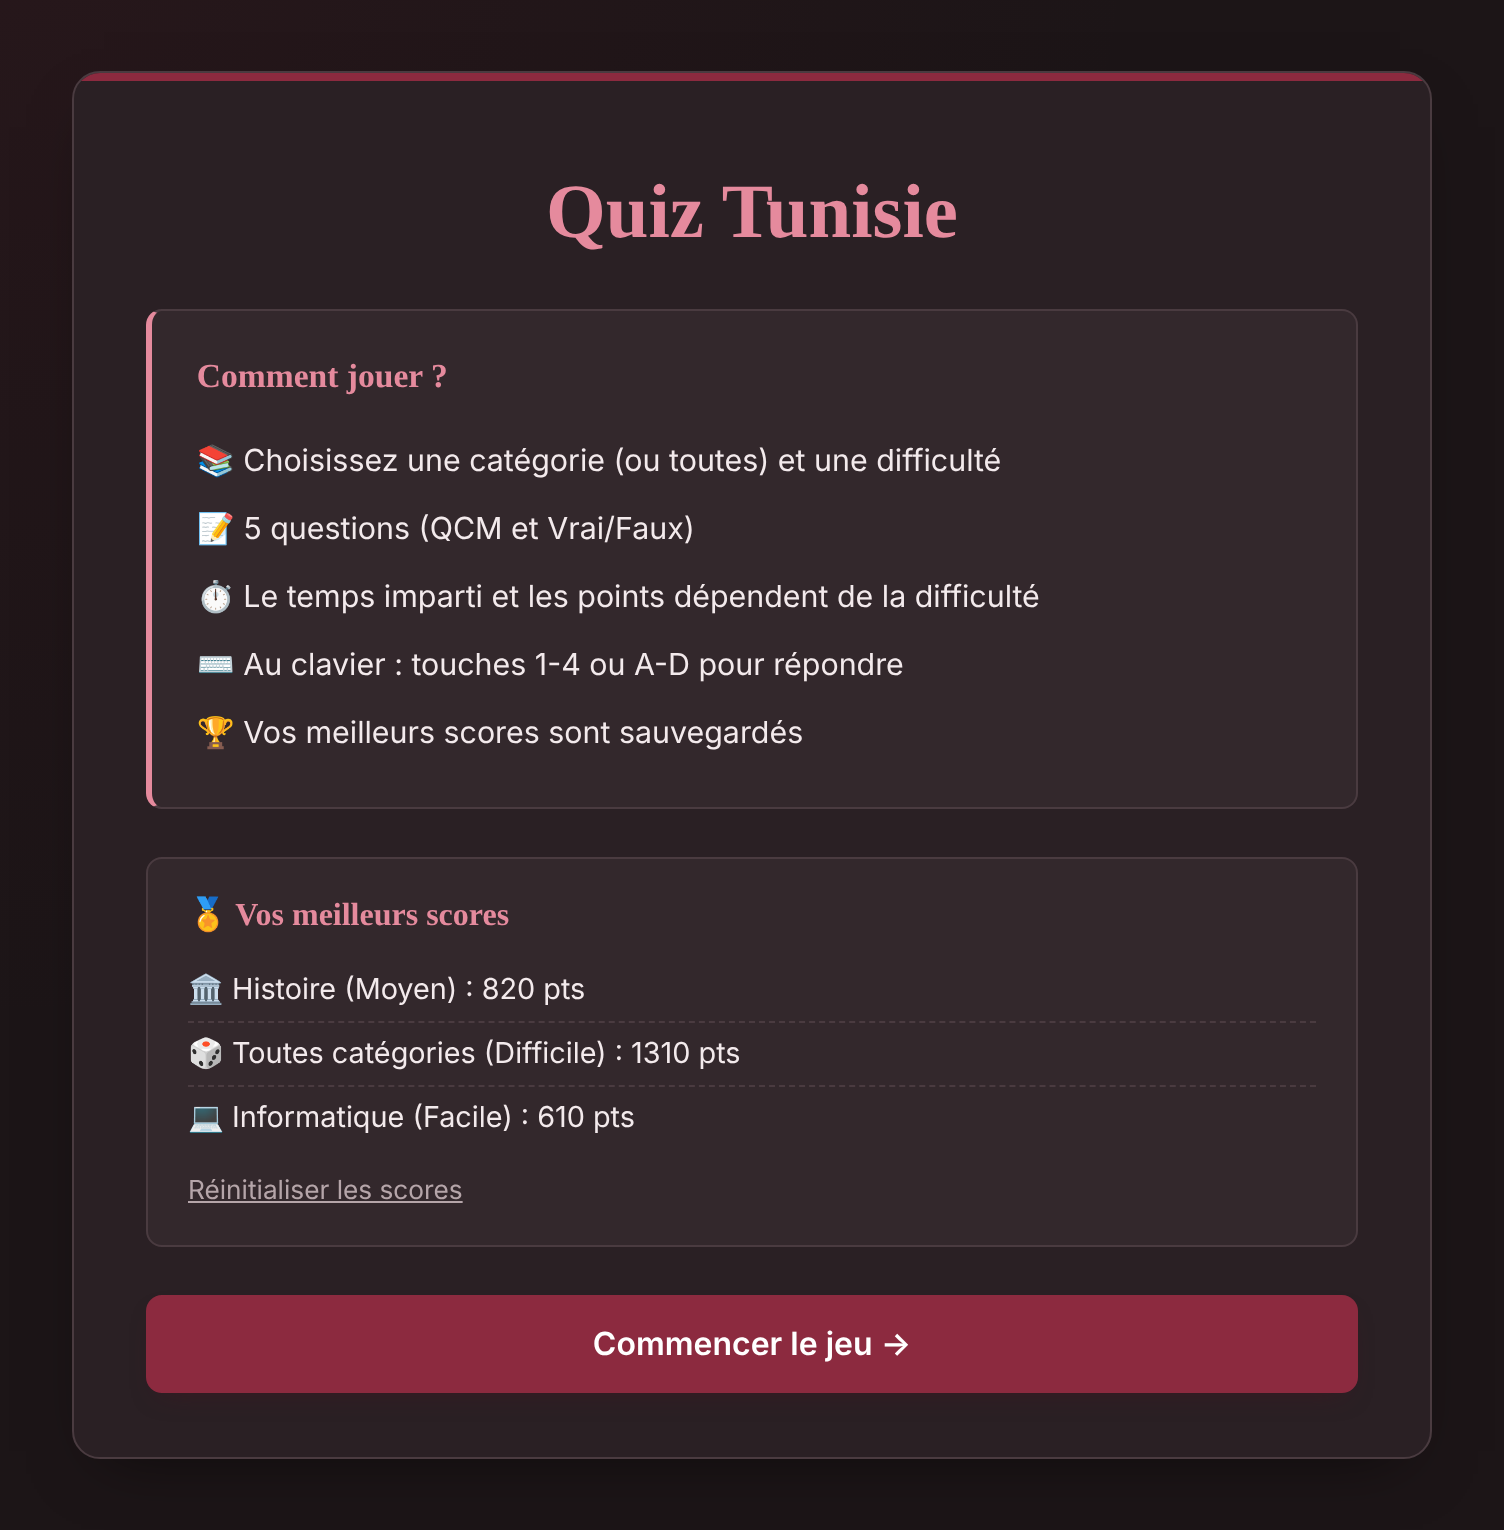
\includegraphics[width=0.46\linewidth]{../images/theme_sombre_accueil.png}}\hfill
  \fcolorbox{bordurecode}{white}{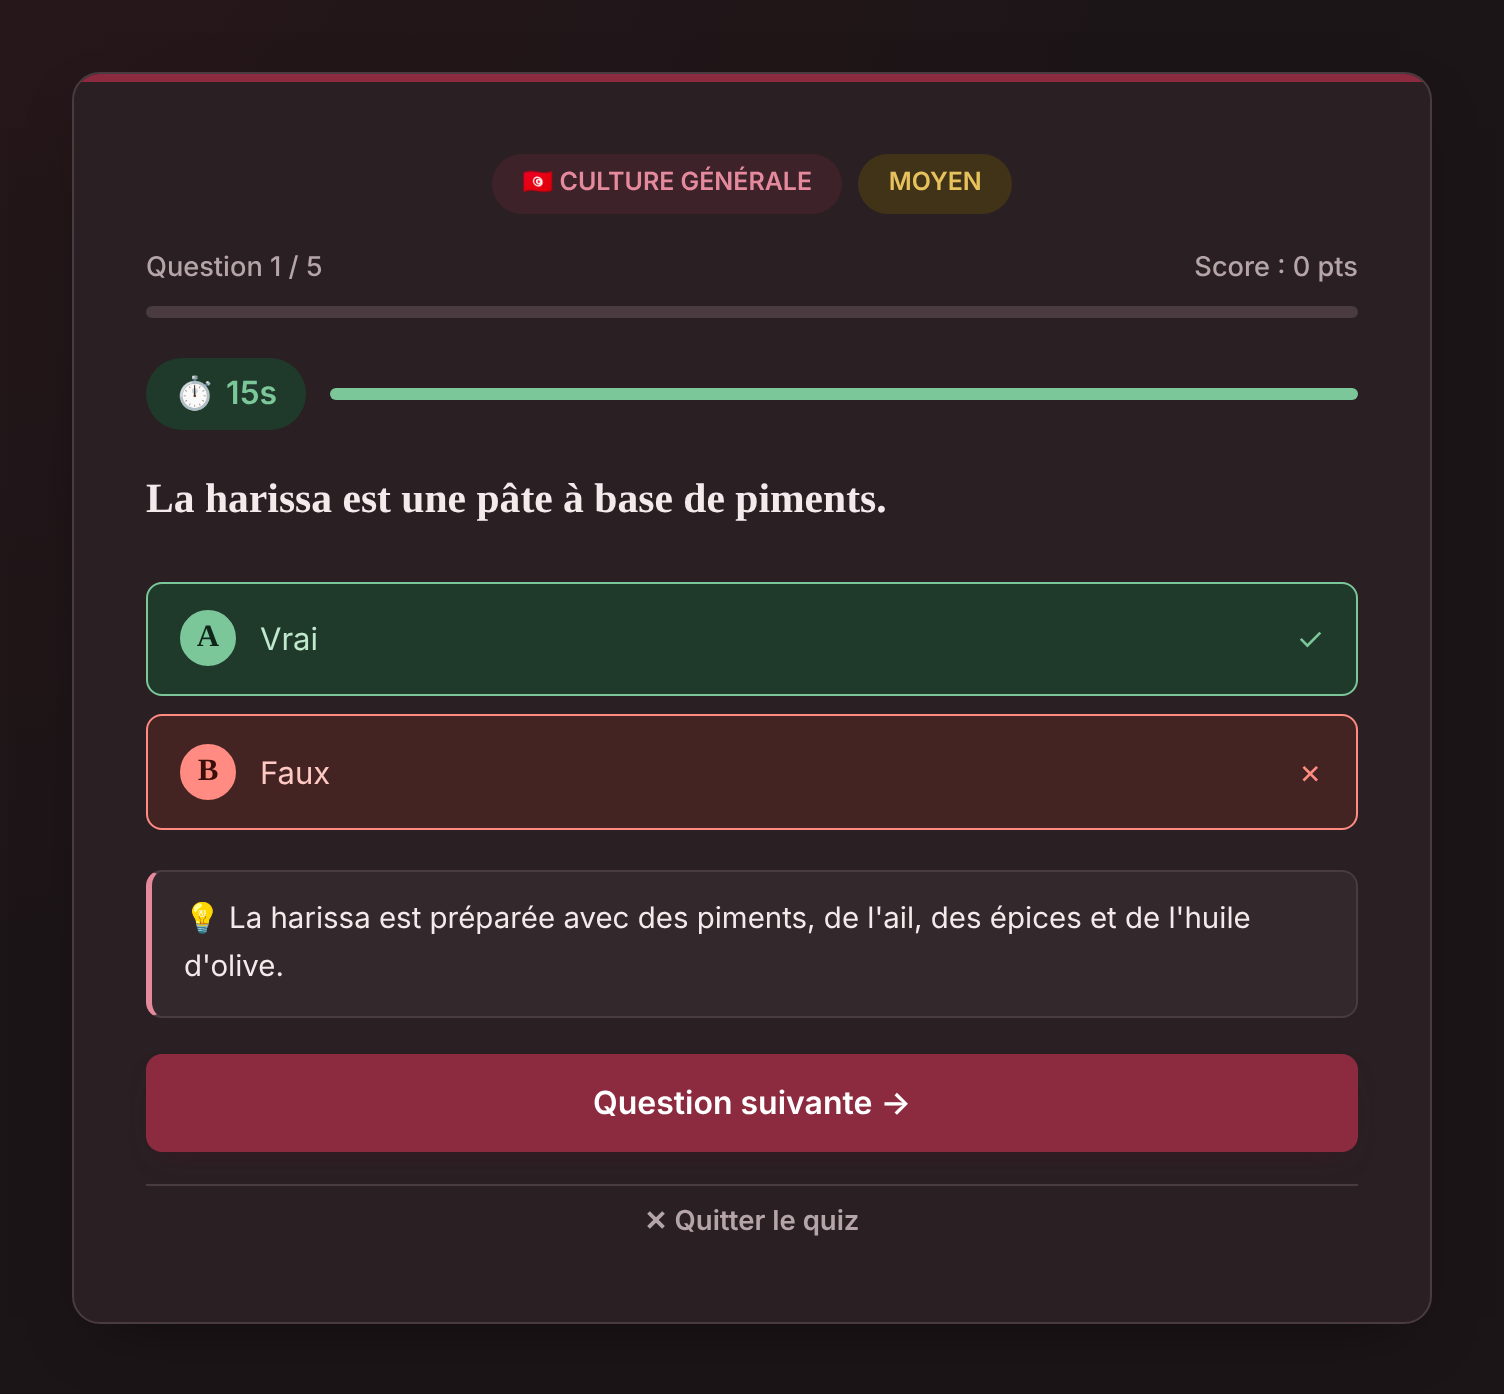
\includegraphics[width=0.46\linewidth]{../images/theme_sombre.png}}
  \caption{Thème sombre automatique (accueil et question).}
\end{figure}

\begin{figure}[H]
  \centering
  \fcolorbox{bordurecode}{white}{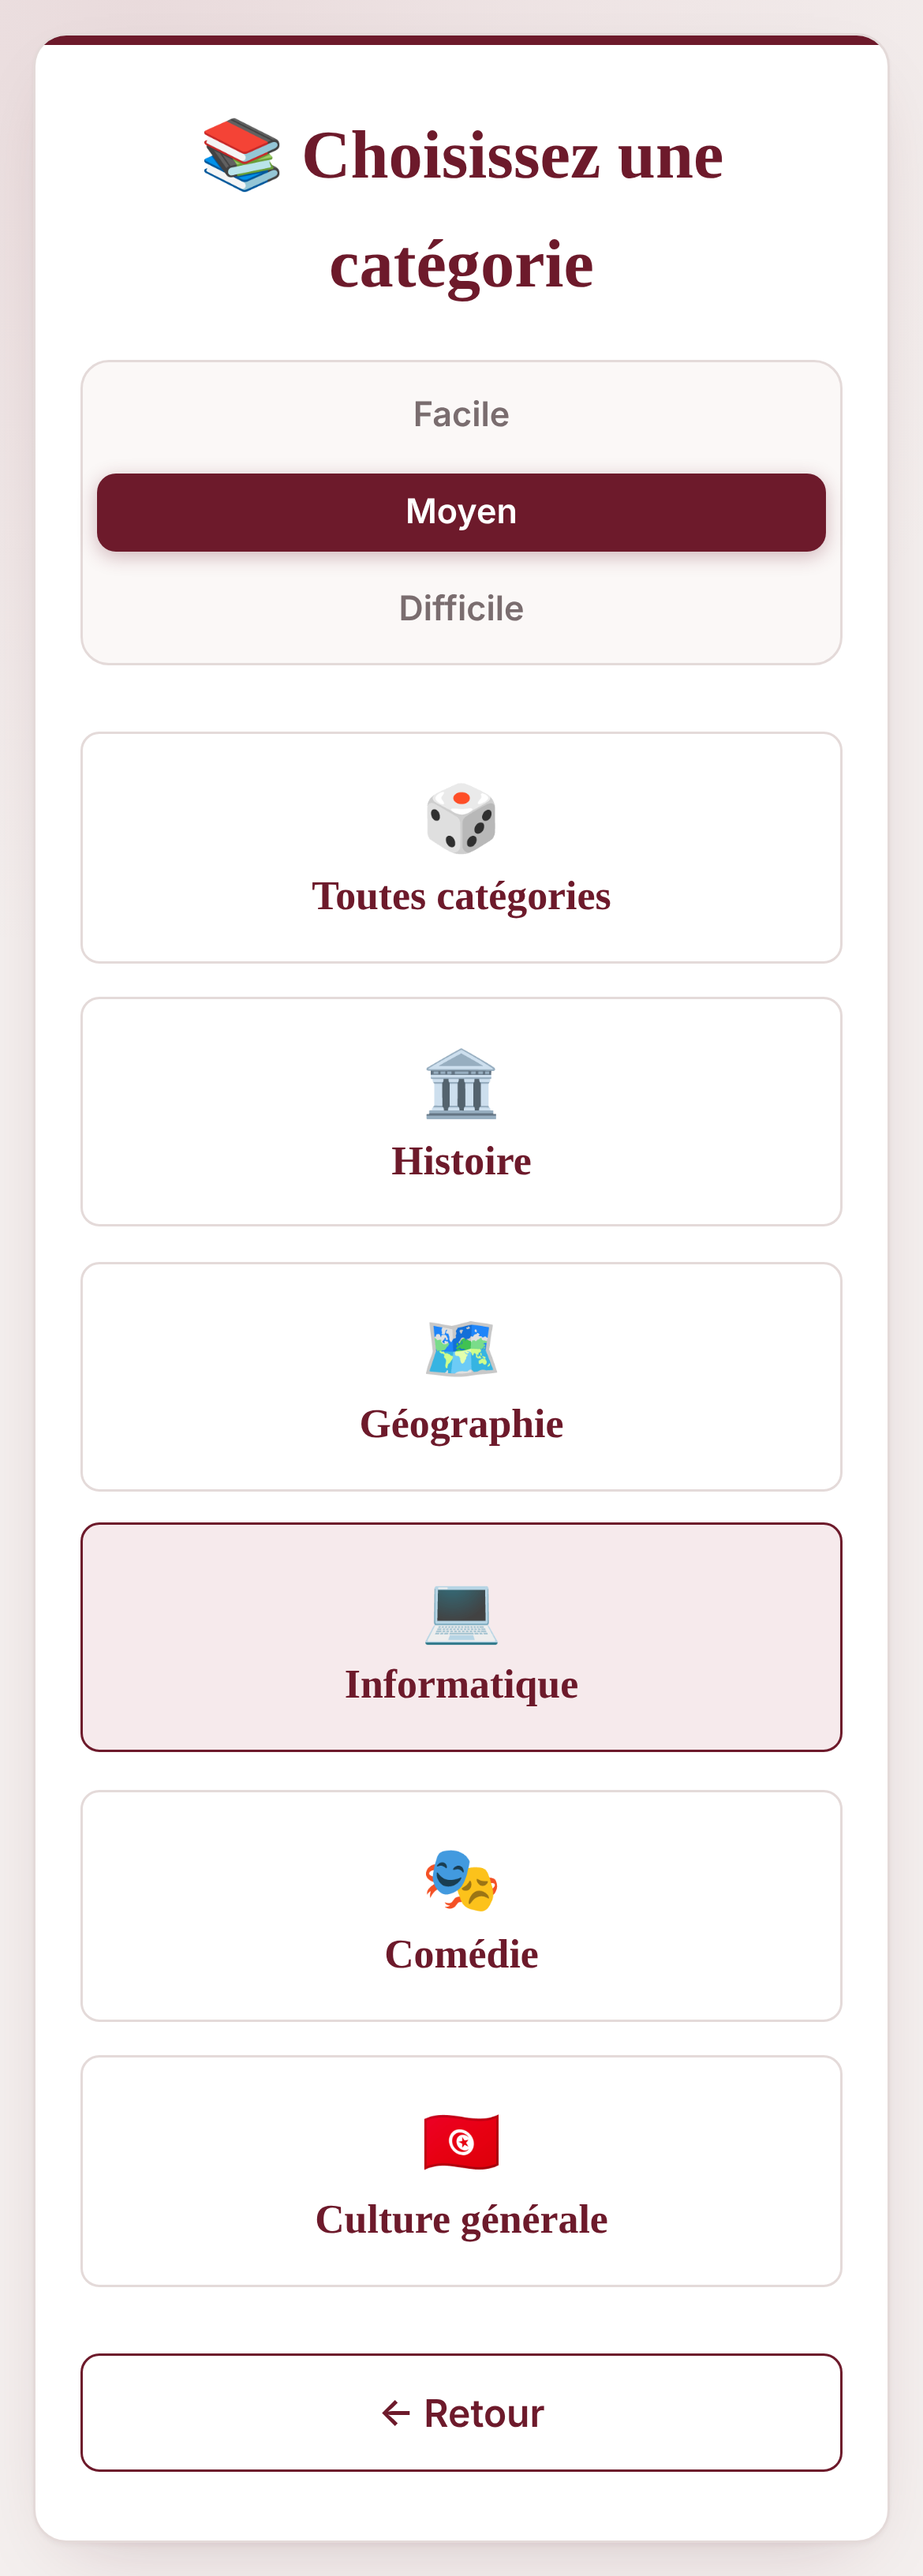
\includegraphics[height=10.5cm]{../images/mobile_categories.png}}\hspace{1cm}
  \fcolorbox{bordurecode}{white}{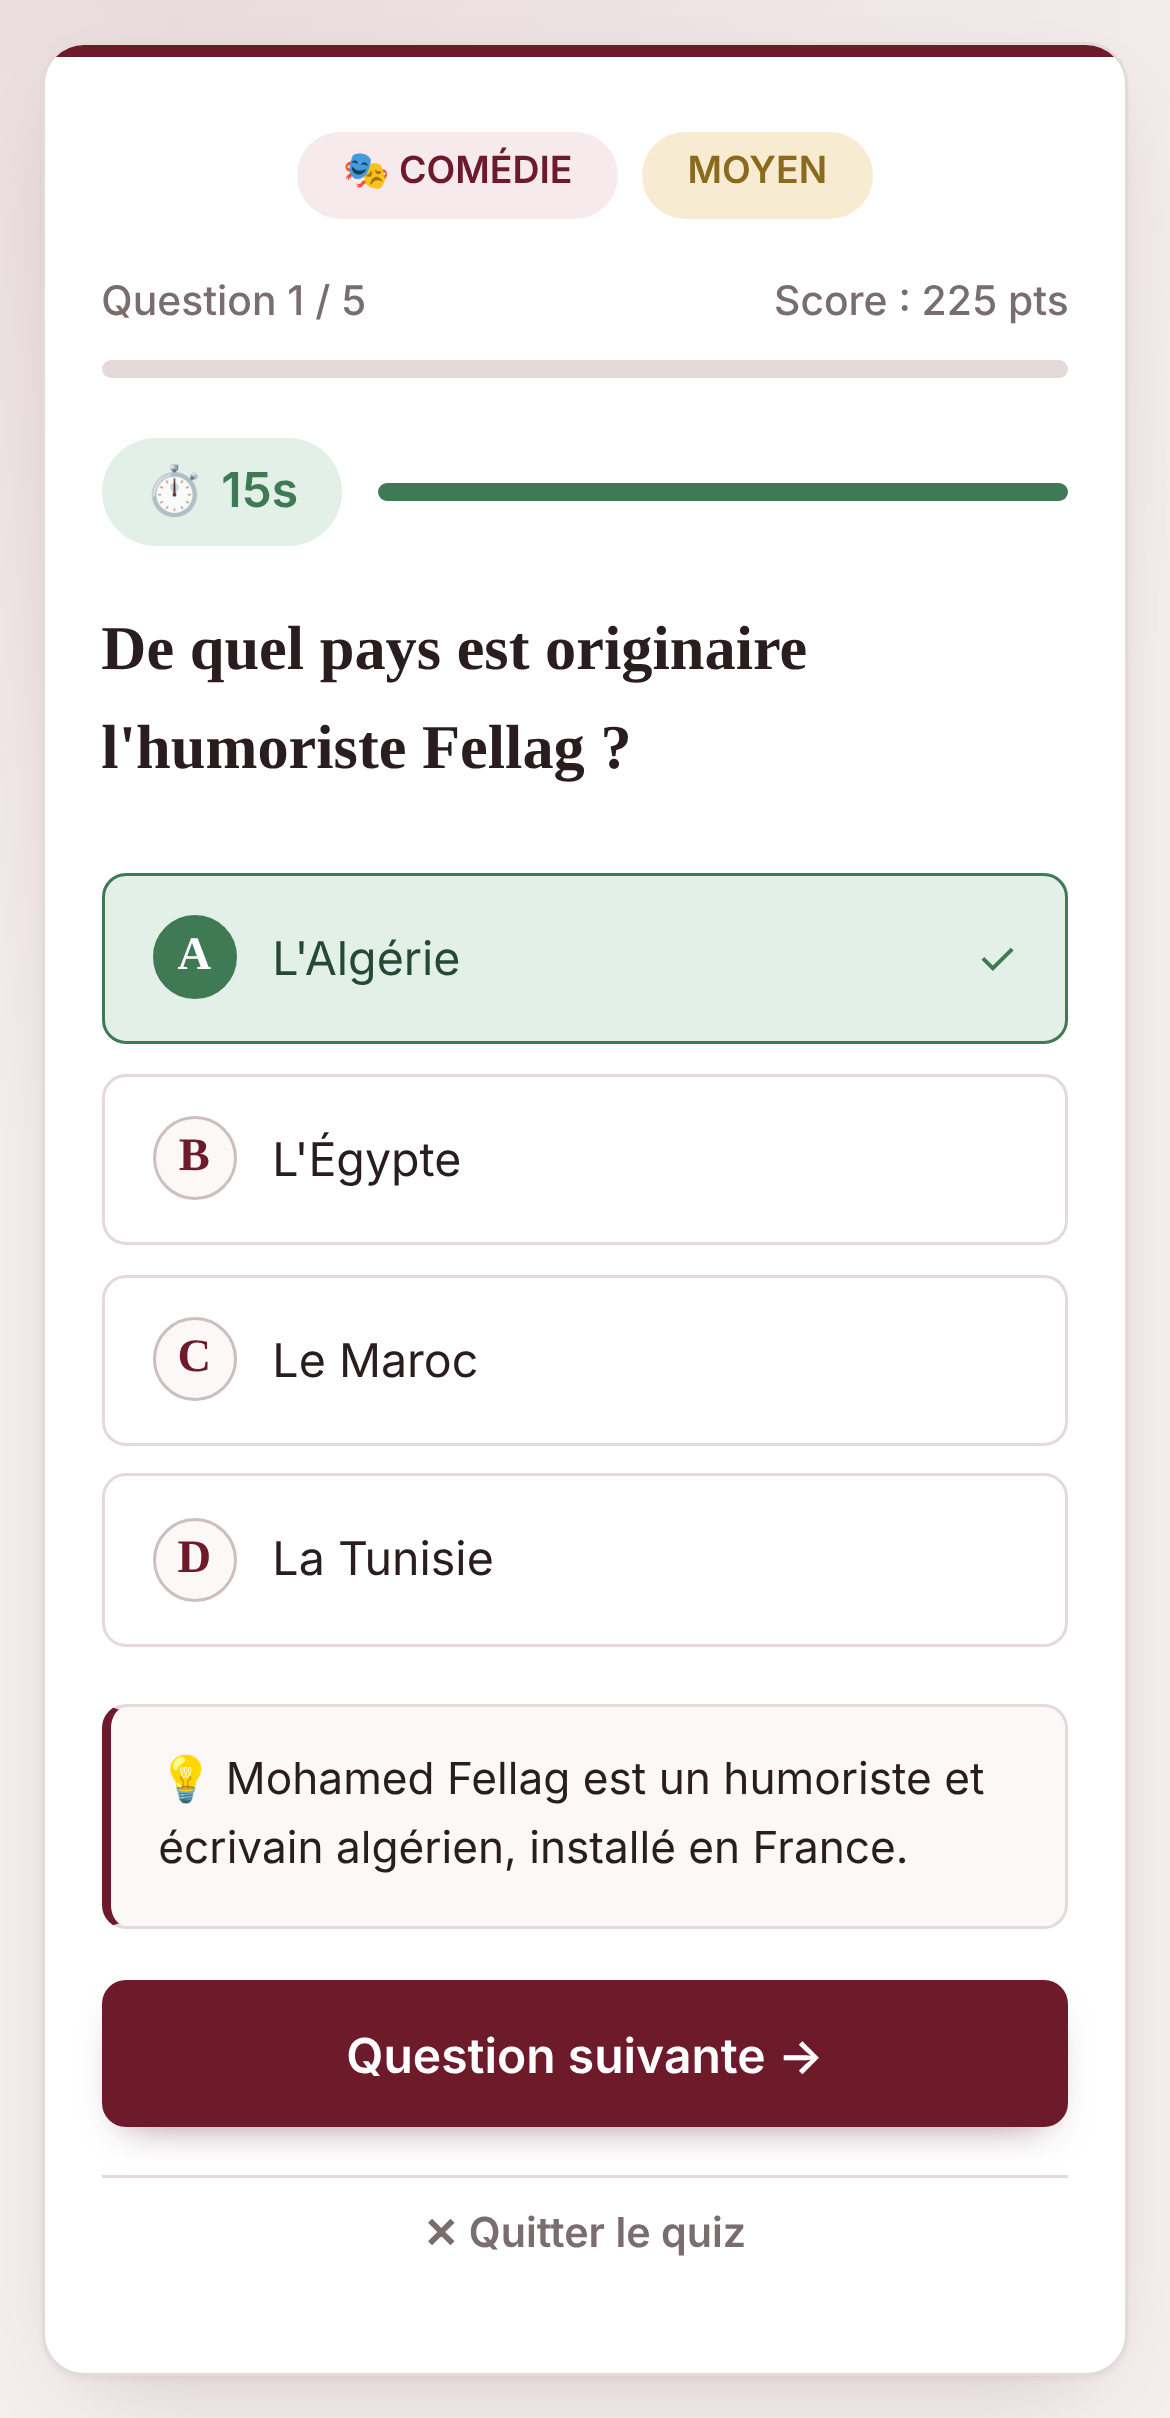
\includegraphics[height=10.5cm]{../images/mobile_question.png}}
  \caption{Version mobile (390 px) : catégories en une colonne et question.}
\end{figure}

\paragraph{Vidéo de démonstration.} Une vidéo d'environ une minute montre une partie
complète : choix de la difficulté et de la catégorie, réponses, chronomètre, résultats et
meilleurs scores. Scannez le QR code avec un téléphone pour la regarder.

\begin{figure}[H]
  \centering
  \begin{minipage}[c]{0.55\linewidth}\centering
    \fcolorbox{bordurecode}{white}{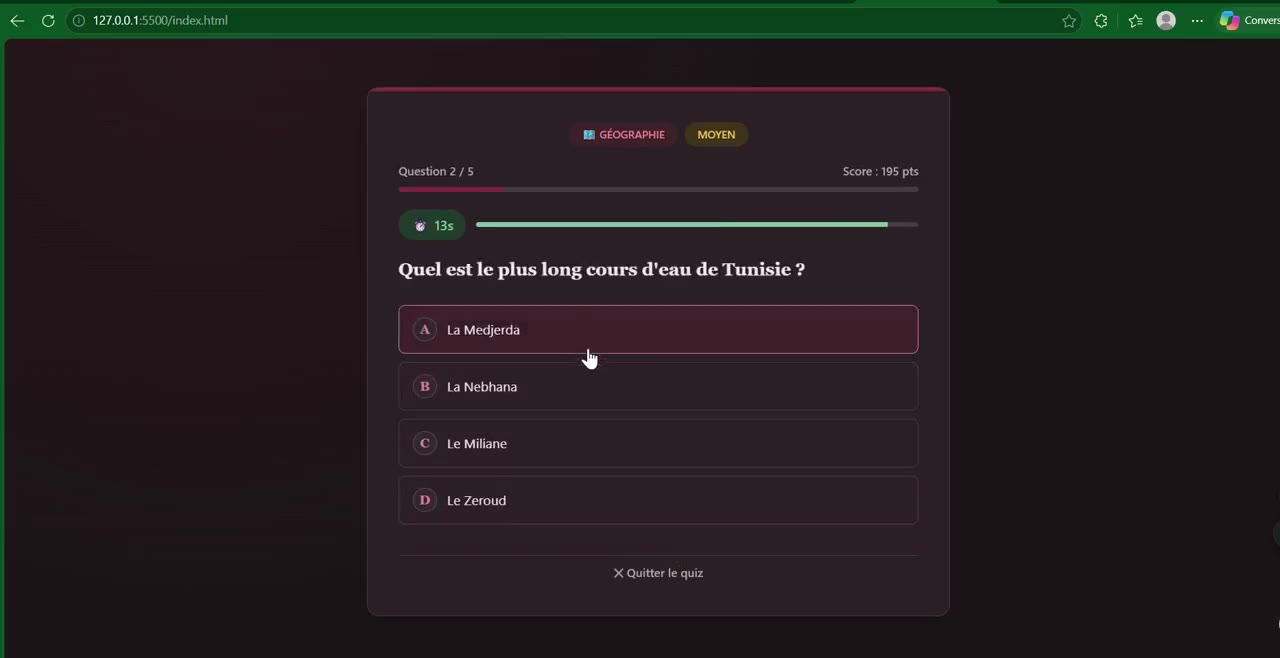
\includegraphics[width=0.95\linewidth]{../images/video_apercu.jpg}}
  \end{minipage}\hfill
  \begin{minipage}[c]{0.4\linewidth}\centering
    \fcolorbox{bordeaux}{white}{\rule{0pt}{0pt}\hspace{2pt}\qrcode[height=4cm]{https://github.com/faten1111/mini_projet_dev/blob/main/demo/demo_quiz.mp4}\hspace{2pt}\rule{0pt}{0pt}}\\[6pt]
    {\small\textcolor{bordeaux}{\textbf{Scannez pour voir la vidéo}}}\\[2pt]
    {\scriptsize\color{grisclair}\url{https://github.com/faten1111/mini_projet_dev/blob/main/demo/demo_quiz.mp4}}
  \end{minipage}
  \caption{Vidéo de démonstration du quiz (QR code vers la vidéo).}
\end{figure}

\subsection{Commentaire du rendu}
La mise en page repose sur une \textbf{carte centrale unique}, bordée d'une fine bande
bordeaux, qui recentre l'attention sur le contenu. La \textbf{cohérence visuelle} est assurée
par une palette restreinte (bordeaux, blanc cassé, vert, ambre, rouge) et une typographie
mixte (sérif pour les titres, sans-serif pour le corps). Les trois couleurs de feedback sont
réutilisées partout : chronomètre, barre de temps et badges de difficulté.

Le \textbf{responsive design} a été testé sur ordinateur (> 600 px) et sur mobile
(< 600 px, notamment 390 px). En dessous de 600 px, la grille de catégories passe d'une
disposition automatique (\texttt{auto-fit}) à une seule colonne, le sélecteur de difficulté
s'empile verticalement et les statistiques de résultats passent de trois colonnes à trois
lignes. Les boutons occupent toute la largeur disponible pour rester accessibles au pouce.

Le \textbf{thème sombre} suit automatiquement le réglage du système d'exploitation ; les
contrastes ont été ajustés (bordeaux éclairci \texttt{\#E58A9D} pour les titres, textes
clairs sur fond foncé).

Les animations restent discrètes : fondu à l'apparition d'un écran, glissement de chaque
nouvelle question, secousse sur une mauvaise réponse, battement du chronomètre en zone rouge
et du message « Nouveau record ». Le tout est désactivé lorsque
\texttt{prefers-reduced-motion} est activé.

\textbf{Lien de démonstration.} (GitHub Pages)
\url{https://faten1111.github.io/mini_projet_dev/}

\subsection{Validation du code (W3C)}
Afin de garantir la qualité, l'interopérabilité et la conformité de notre application aux
standards du web, l'ensemble des fichiers sources de cette nouvelle version a été soumis
aux validateurs officiels du World Wide Web Consortium (W3C).
\begin{itemize}
  \item \textbf{Validation HTML5} : le fichier \texttt{index.html} a été analysé avec le
        \textbf{Nu Html Checker} (vnu 26.11.4). Le résultat indique « \textit{Document
        checking completed. No errors or warnings to show.} » (aucune erreur ni
        avertissement).
  \item \textbf{Validation CSS3} : le fichier \texttt{style.css} a été vérifié par le
        \textbf{W3C CSS Validation Service} (CSS niveau 3 + SVG). Le validateur affiche
        « \textit{Félicitations ! Aucune erreur trouvée.} ». Les 20 avertissements signalés
        ne sont pas des erreurs : ils concernent principalement l'usage des variables CSS et de propriétés
        préfixées (\texttt{-webkit-font-smoothing}), que le validateur ne peut pas vérifier
        statiquement.
  \item \textbf{Validation JavaScript} : les fichiers \texttt{questions.js} et
        \texttt{script.js} ont été vérifiés avec \textbf{Node.js} (commande
        \texttt{node --check} et petit script \texttt{validate.js}) : les deux fichiers
        sont analysés sans aucune erreur de syntaxe (« parses cleanly »).
\end{itemize}

Les captures d'écran ci-dessous attestent de ces validations :

\capture{html_validation.png}{0.95\linewidth}{Validation HTML5 --- Nu Html Checker (0 erreur, 0 avertissement).}
\capture{css_validation.png}{0.95\linewidth}{Validation CSS3 --- W3C CSS Validator (aucune erreur trouvée).}
\capture{js_validation.png}{0.85\linewidth}{Validation JavaScript --- analyse syntaxique avec Node.js (0 erreur).}

\subsection{Audit de qualité (Lighthouse)}
En complément des validateurs W3C, l'application a été analysée avec \textbf{Lighthouse},
l'outil d'audit intégré aux outils de développement de Google Chrome (onglet
\textit{Lighthouse}). L'audit a été lancé sur la page servie localement par Live Server
(\texttt{http://127.0.0.1:5500/index.html}). Il évalue quatre critères :
\begin{itemize}
  \item \textbf{Performance : 100 / 100} --- la page s'affiche très rapidement
        (\textit{First Contentful Paint} et \textit{Largest Contentful Paint} de
        0,3 s), grâce à l'absence de framework et de ressources externes lourdes ;
  \item \textbf{Accessibilité : 100 / 100} --- contrastes suffisants, rôles et attributs
        ARIA corrects, boutons nommés, langue de la page déclarée (\texttt{lang="fr"}) ;
  \item \textbf{Bonnes pratiques : 100 / 100} --- aucune erreur dans la console, pas
        d'API obsolète, code JavaScript sans \texttt{innerHTML} ;
  \item \textbf{SEO : 100 / 100} --- balises \texttt{<title>} et
        \texttt{<meta name="description">} présentes, balise \texttt{viewport} adaptée
        au mobile.
\end{itemize}

\capture{lighthouse.png}{0.75\linewidth}{Audit Lighthouse --- 100 / 100 en performance, accessibilité, bonnes pratiques et SEO.}

% =========================================================
\clearpage
\section{Améliorations par rapport à la première version}
% =========================================================
\begin{table}[H]
\centering
\renewcommand{\arraystretch}{1.3}
\small
\begin{tabularx}{\linewidth}{@{}>{\bfseries}p{3.2cm} X X@{}}
\toprule
Aspect & Version 1 & Version 2 (actuelle) \\
\midrule
Fichiers & 3 fichiers, questions dans \texttt{script.js} & 4 fichiers : données séparées dans \texttt{questions.js} \\
Organisation du code & Fonctions + objet global \texttt{state} & 3 classes ES6 (\texttt{ScoreManager}, \texttt{QuizTimer}, \texttt{QuizGame}) \\
Catégories & 5 catégories & 5 catégories + mode « Toutes catégories » \\
Questions & 35 QCM & 50 questions : QCM et Vrai / Faux, avec niveau et explication \\
Difficulté & Aucune (15 s fixes) & Facile 20 s / Moyen 15 s / Difficile 10 s \\
Score & 1 point par bonne réponse & Points selon le niveau + bonus de rapidité (jusqu'à +50 \%) \\
Chronomètre & Relancé à 15 s au retour sur l'onglet & Vraie pause / reprise, barre de temps, alertes à 50 \% et 20 \% \\
Après la réponse & Couleurs vert / rouge & Couleurs + explication de la bonne réponse \\
Résultats & Score, statistiques & + nouveau record, récapitulatif « À revoir » \\
Meilleurs scores & Non & Oui, par catégorie et difficulté (\texttt{localStorage}) \\
Clavier & Tabulation uniquement & Touches 1--4 / A--D, Entrée pour continuer \\
Thème & Clair uniquement & Clair + sombre automatique \\
Quitter & Immédiat & Confirmation avant de perdre la partie \\
\bottomrule
\end{tabularx}
\caption{Comparaison entre la première et la deuxième version.}
\end{table}

% =========================================================
\section{Difficultés rencontrées et solutions}
% =========================================================
\begin{table}[H]
\centering
\renewcommand{\arraystretch}{1.35}
\small
\begin{tabularx}{\linewidth}{@{}>{\raggedright\arraybackslash}p{5cm} X@{}}
\toprule
\textbf{Difficulté} & \textbf{Solution apportée} \\
\midrule
Alignement horizontal du chronomètre et de sa barre de temps & Flexbox (\texttt{display:flex}, \texttt{gap}) avec une barre \texttt{flex:1} \\
Mauvais rendu sur mobile & Media query à 600 px : grille sur une colonne, sélecteur de difficulté vertical, statistiques en lignes \\
Chronomètre qui continue en arrière-plan, puis qui repartait de zéro & Événement \texttt{visibilitychange} + classe \texttt{QuizTimer} avec \texttt{pause()} / \texttt{resume()} qui conserve le temps restant \\
Double sélection de réponse (double-clic rapide ou touche clavier) & Drapeau \texttt{isAnswered} et \texttt{button.disabled = true} \\
Ordre des réponses prévisible & Mélange Fisher--Yates des QCM ; ordre fixe pour les Vrai/Faux (plus naturel) \\
Pas assez de questions d'un niveau dans une catégorie & Tri par écart de niveau : on complète avec les niveaux les plus proches \\
Changement de difficulté pendant une partie & Paramètres figés dans \texttt{startGame()} (\texttt{activeDifficulty}, \texttt{maxTime}, \texttt{basePoints}) \\
\texttt{localStorage} indisponible ou données corrompues & Lecture/écriture dans des blocs \texttt{try / catch}, valeur par défaut \texttt{\{\}} \\
Couleurs illisibles en thème sombre & Toutes les couleurs en variables CSS, redéfinies dans \texttt{prefers-color-scheme: dark} \\
Animation qui ne se relance pas à chaque question & Suppression puis remise de l'animation avec un \textit{reflow} forcé (\texttt{offsetWidth}) \\
Contraste insuffisant de certains textes & Variables dédiées (\texttt{--vert-ok-texte}, \texttt{--rouge-ko-texte}) et vérification avec un contrôleur de contraste \\
\bottomrule
\end{tabularx}
\caption{Difficultés techniques et solutions.}
\end{table}

% =========================================================
\clearpage
\section{Conclusion}
% =========================================================
Ce mini-projet nous a permis de consolider nos connaissances en HTML5, CSS3 et
JavaScript natif, en particulier :
\begin{itemize}
  \item la structuration sémantique d'une page web (rôles ARIA, sections, en-têtes) ;
  \item la mise en page responsive combinant Flexbox et CSS Grid et l'usage raisonné des
        media queries ;
  \item l'utilisation des variables CSS pour gérer un thème clair et un thème sombre ;
  \item la programmation orientée objet en JavaScript (classes, responsabilités séparées)
        et la séparation des données et de la logique ;
  \item la manipulation du DOM, la gestion d'état côté client et la persistance des
        données avec le \texttt{localStorage} ;
  \item la création d'animations CSS discrètes et respectueuses des préférences
        d'accessibilité ;
  \item la validation W3C, l'audit Lighthouse (100 / 100 sur les quatre critères) et le
        souci du contraste et de l'ergonomie (clavier, lecteurs d'écran).
\end{itemize}

L'ensemble constitue une base solide pour aborder le développement web dynamique
(frameworks JS, appels HTTP, back-end) lors des projets futurs. Les perspectives
d'évolution incluent l'ajout d'un \textbf{mode multijoueur}, d'un \textbf{classement en
ligne} partagé (via une API), d'un \textbf{éditeur de questions} pour permettre aux
enseignants de créer leurs propres quiz, et d'une version bilingue (français / arabe).

% =========================================================
\clearpage
\appendix
\section{Annexes}
% =========================================================
\subsection{Code complet --- fichier \texttt{index.html}}
\lstinputlisting[language=HTML]{code/index.html}

\subsection{Code complet --- fichier \texttt{style.css}}
\lstinputlisting[language=CSS]{code/style.css}

\subsection{Code complet --- fichier \texttt{questions.js}}
\lstinputlisting[language=JavaScript]{code/questions.js}

\subsection{Code complet --- fichier \texttt{script.js}}
\lstinputlisting[language=JavaScript]{code/script.js}

\subsection{Ressources et documentation}
\begin{itemize}
  \item MDN Web Docs --- HTML, CSS, JavaScript (\url{https://developer.mozilla.org/fr/}) ;
  \item MDN --- Classes JavaScript, \texttt{localStorage}, \texttt{prefers-color-scheme} ;
  \item W3C Markup Validation Service (\url{https://validator.w3.org/}) ;
  \item W3C CSS Validation Service (\url{https://jigsaw.w3.org/css-validator/}) ;
  \item WAI-ARIA Authoring Practices --- motif « radio group » (\url{https://www.w3.org/WAI/ARIA/apg/}) ;
  \item Polices système : Georgia et Segoe UI.
\end{itemize}

\end{document}
